\documentclass[a4paper,10pt,american]{article}
\usepackage[top=1in, bottom=1in, left=0.75in, right=0.75in]{geometry}
\usepackage{amsmath,amssymb,amsfonts,mathrsfs,accents} %important math packages
\usepackage{graphicx}
\usepackage{subcaption}
% \usepackage{float}
\usepackage{bbm}
\usepackage{dsfont}
\usepackage{tikz}
\usepackage{enumerate} % package for making different lists
\usepackage[T1]{fontenc} % Encoding of fonts
\usepackage{lmodern} % Latin modern font - needed for fontenc
\usepackage[utf8]{inputenc} % Encoding of input text
\usepackage[kerning]{microtype} % Better looking text
\usepackage[babel]{csquotes} % Better looking quotes
\usepackage{booktabs} % Better looking tables
\usepackage{babel} % Language control, for hyphenation etc
\usepackage{amsthm} % Package for theorem and definition environments
\usepackage{hyperref} % URLs 
\usepackage{comment}
\usepackage{xcolor}
\usepackage{amsmath}
\usepackage[table]{xcolor}
\usepackage{istgame}
\usepackage{mathpazo} % Other fonts: lmodern & charter & mathptmx
% \usepackage{minted}
% \usemintedstyle{colorful}  % Choose a highlighting style
\usepackage{listings}
% Package for drawing in Latex. Depending on your installation you might need compat=1.12 or 1.11 uncommented.  
\usepackage{tikz}
\usetikzlibrary{calc}
\usetikzlibrary{trees}
\usepackage{pgfplots}
\usepackage{fancyhdr}
\usepackage{footmisc}
%\pgfplotsset{compat=1.12}
\pgfplotsset{compat=1.11}

% For better figure placement in documents. Use [H] instead of the usual [htbp]. Inserted at the same place as in the code, as you normally want it to. 
\usepackage{float}

% Row break instead of indent for new paragraph. 
\usepgfplotslibrary{fillbetween}
\setlength{\parskip}{10pt plus 1pt minus 1pt}
\setlength{\parindent}{0in}

% Define Stata language style
\lstdefinelanguage{Stata}{
    morekeywords={regress, gen, summarize, predict, display, if, forval, local, matrix},
    sensitive=true,
    morecomment=[l]{*},
    morestring=[b]",
}
% Set listings style
\lstset{
    language=Stata,
    basicstyle=\ttfamily\small,    % Code font
    keywordstyle=\color{blue},    % Keywords in blue
    commentstyle=\color{gray},    % Comments in gray
    stringstyle=\color{red},      % Strings in red
    breaklines=true,              % Allow line breaking
    numbers=left,                 % Line numbers on the left
    numberstyle=\tiny\color{gray},
    frame=single,                 % Frame around the code
    captionpos=b,                 % Caption position
}
% Examples of personal commands to simplify writing stuff you use often. 
\newcommand{\reals}{\mathbb{R}} 
\newcommand{\rtwo}{\mathbb{R}^2}
\newcommand{\ints}{\mathbb{Z}}
\newcommand{\nats}{\mathbb{N}}
\newcommand{\matset}{\mathcal{M}}
\newcommand{\zerovec}{\{\mathbf{0}\}}
% \renewcommand{\footnoterule}{%
%     \kern 210pt
%     \hrule width \textwidth height 0.4pt
%     \kern 2.6pt
% }
\definecolor{navy}{RGB}{0, 0, 128}
\hypersetup{
    colorlinks=true,
    linkcolor=navy,
    filecolor=navy,
    urlcolor=navy,
    citecolor=navy,
}
\title{Asset Pricing Theory --- Problem Set 4}
% \thanks{
%     The latest version of this document and related 
%     materials can be accessed at: 
%     \href{https://github.com/AliBahramiSani/TAP_Com_Crsp_CAPM.git}{Github Repository}.
% }
\author{Ali Bahramisani\thanks{Stockholm School
of Economics, Department of Finance, Email: 
\href{mailto:ali.bahramisani@hhs.se}{ali.bahramisani@hhs.se}, Website: \href{https://alibahramisani.github.io}{alibahramisani.github.io}}}
 
%, Website: \href{https://alibahramisani.github.io}{alibahramisani.github.io}
\date{Spring 2025}
% Version: \today
\pagestyle{fancy}
\fancyhf{}
\fancyhead[L]{Ali Bahramisani}
\fancyhead[C]{Asset Pricing Theory -- Spring 2025}
\fancyhead[R]{Problem Set 4}
\fancyfoot[C]{\thepage}
% \setlength{\abovecaptionskip}{0pt}
% \setlength{\belowcaptionskip}{0pt}

% \usepackage{natbib}
% \bibliographystyle{abbrvnat}
% \setcitestyle{authoryear,open={(},close={)}}

\begin{document}
\maketitle
% \vspace{1cm}
%     \begin{center}
%         \includegraphics[width=0.9\textwidth]{DG.jpg} \\[1ex]
%         {\footnotesize \textit{David With the Head of Goliath and two Soldiers} \citep{valentin_boulogne_david}. 
%         David outperformed his large enemy, but at a great risk.}
%     \end{center}
%     \vfill
\thispagestyle{empty}



\newpage
\pagenumbering{arabic}

\section{Optimization}
In this section, I use the first order taylor approximation for the Newton-Raphson method to solve the problem.

\subsection{A Polynomial}
I tried to solve the problem with Newton-Raphson iteration method, as well as using Python built in solvers. The results are presented in \autoref{fig:poly}.

\begin{figure}[H]
\centering
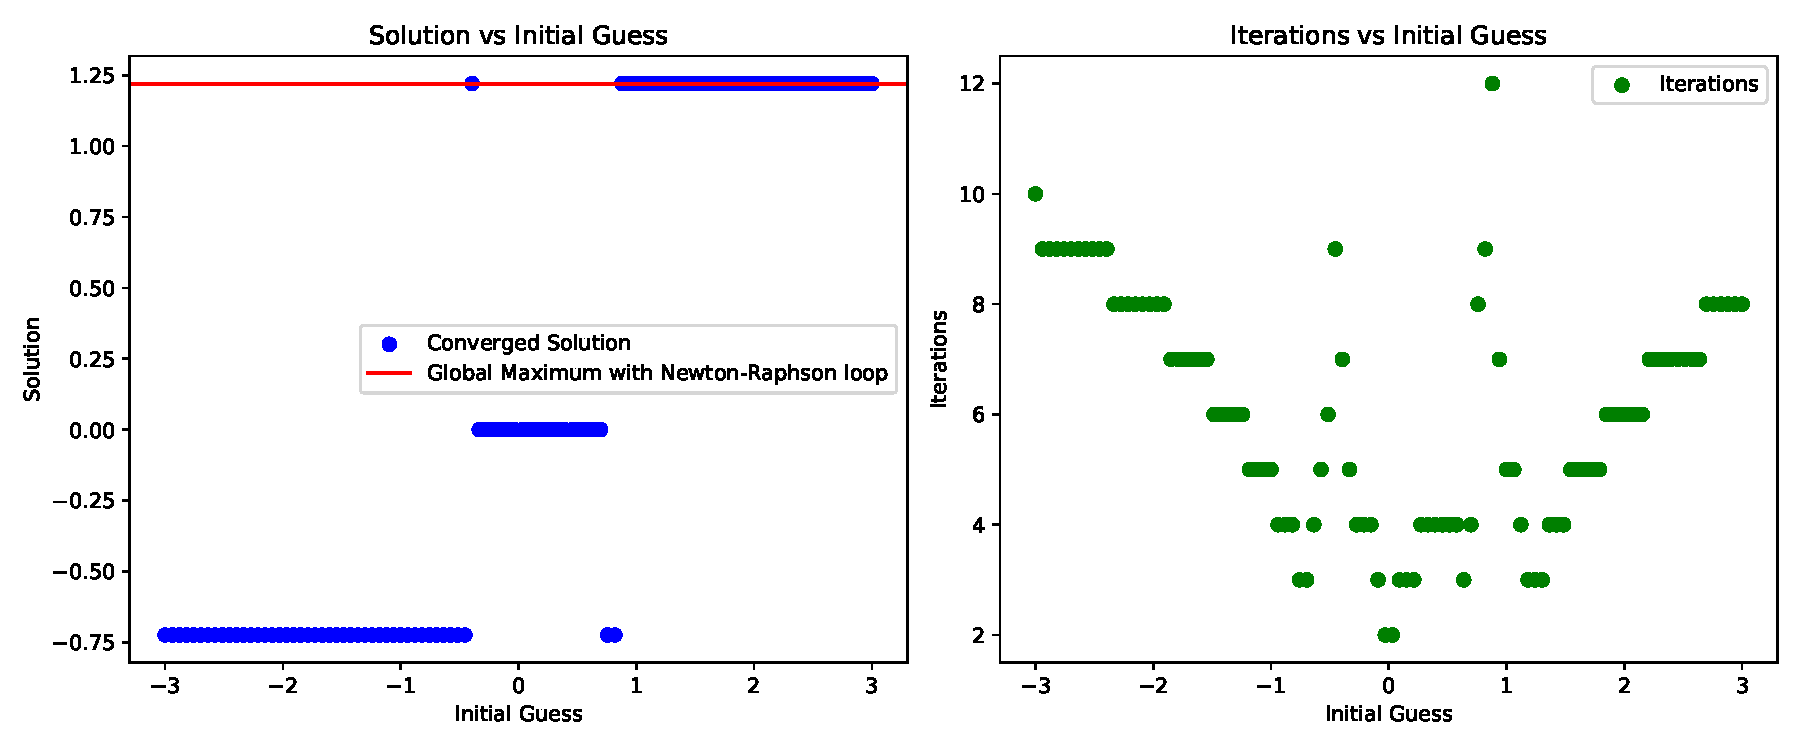
\includegraphics[width=1\linewidth]{../Plots/NR_X0.pdf}
\caption{Obtained solution and the number of iterations against the initial guess}
\label{fig:poly}
\end{figure}

As it is shown, the Newton-Raphson method with the first order taylor approximation, conditional on the initial guess, could not precisely solve the problem. Also, since this method is heavily contingent on the local derivations, the initial guess is crucial for the convergence and the solution. We can see that as the initial guess is closer to the local optimas, the method converges faster to those optimas. However, some of them are not global maximas, and the method converges to those local maximas. Considering the global maximum that Newton-Raphson method converges to, only $37\%$ of intitial guesses converge to the global maximum. 

\subsection{The sigmoid function}

The true solution is obviously zero. I, again, wolve the problem with the first order taylor approximation of Newton-Raphson method. The results are presented in \autoref{fig:sigmoid}. As we can see, initial guesses far from the solution are diverging from the true solution. However, the method converges to the true solution for the initial guesses close to the true solution. Initial guesses far from the true solution are diverging due to the fact that for small and high initial guesses, the first derivation of the sigmoind function is extremly large and close to zero, respectively. This makes the Newton-Raphson method to diverge from the true solution.

Put differently, by calculating the average update steps, we can see that the method converges to the true solution for the initial guesses close to the true solution. However, for the initial guesses far from the true solution, the method diverges from the true solution. The average update steps are defined as:
\begin{align}
    \text{Average update steps} = \frac{1}{N} \sum_{i=1}^{N} \left| x_{n+1} - x_{n} \right|
\end{align}
where $N$ is the number of iterations, and $x_{n}$ is the solution at the $n$th iteration. As we can see the average update steps in \autoref{fig:sigmoid}, they are decreasing as the initial guess is closer to the true solution.

\begin{figure}[H]
\centering
\includegraphics[width=1\linewidth]{../Plots/NR_sigmoid.pdf}
\caption{Obtained solution and the average update steps against the initial guess}
\label{fig:sigmoid}
\end{figure}

All in all, combining the results in \autoref{fig:poly} and \autoref{fig:sigmoid}, we can see that the Newton-Raphson method is pretty fast when the initial guess is closer to the true solution. However, for the initial guesses far from the true solution, the method diverges from the true solution. If the function is differentiable this is an easy method to impelement. However, for non-differentiable functions, we cannot use it. In regions that the derivations are close to zero, the method diverges from the true solution. Also, this method maybe useful for local optimization. Finally, the method is contingent on the order of derivations, which as it increases it is more precise, but also more computationally expensive.

\subsection{The bisection algorithm}

It takes $19$ iterations to converge to the solution with the bisection method depicted in \autoref{fig:bisection}. Compare to Newton-Raphson method, bisection method is slower, but guaranteed to find the correct solution. The bisection method is not contingent on the initial guess, and it is not contingent on the derivations of the function. However, it is slower than the Newton-Raphson method. Bisection alwasy find a root!

\begin{figure}[H]
\centering
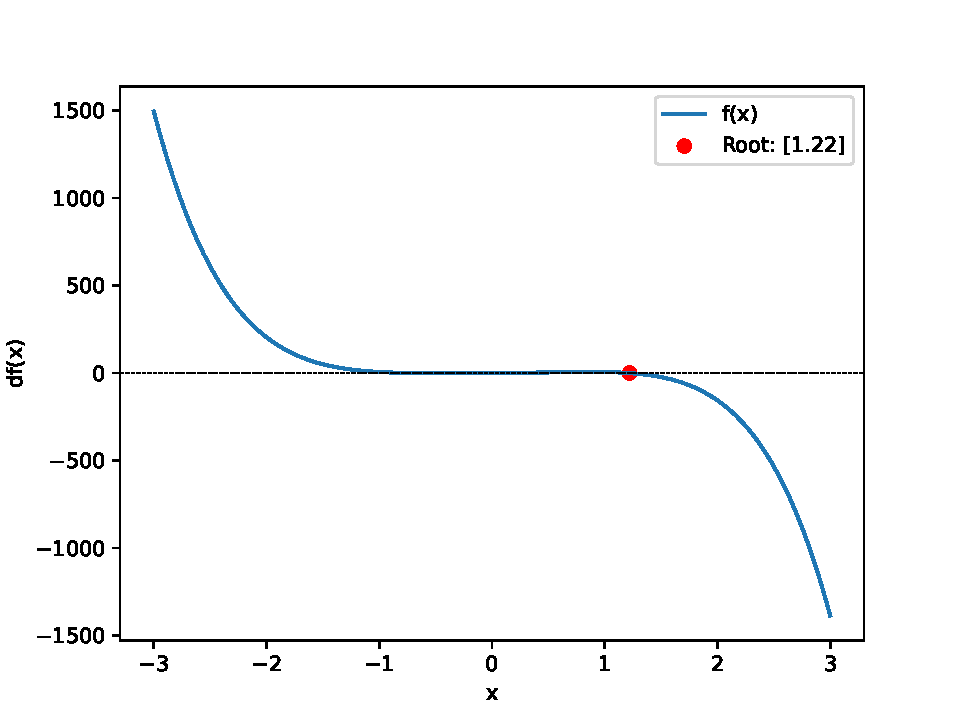
\includegraphics[width=1\linewidth]{../Plots/Bisection.pdf}
\caption{Bisection Method: Roots of $f(x)$}
\label{fig:bisection}
\end{figure}

\newpage
\section{Numerical Integral}
\begin{enumerate}
    \item We have the following for the number of intervals:
    \begin{align}
        |10^{-4}| &\leq \frac{2.57474^3}{12n^2}\cdot 160\to n_{Trapezoidal}\geq 1507\\
        |10^{-4}| &\leq \frac{2.57474^5}{180n^4}\cdot 360\cdot 1.57474^2\to n_{Simpson}\geq 50\text{ It must be even!}
    \end{align}


    \item [2, 3.] The results are presented in \autoref{fig:integrals}. As we can see, the Simpson's method is more precise in lowe iterations, then Trapezoidal method is more precise as $N$ increases. However, for Monte Carlo, it is more dependent on the random process. For instance, we can see with seed $\boldsymbol{137}$, and $1000$ iterations, its error is less than the error of the Simpson's method.
    \begin{figure}[H]
        \centering
        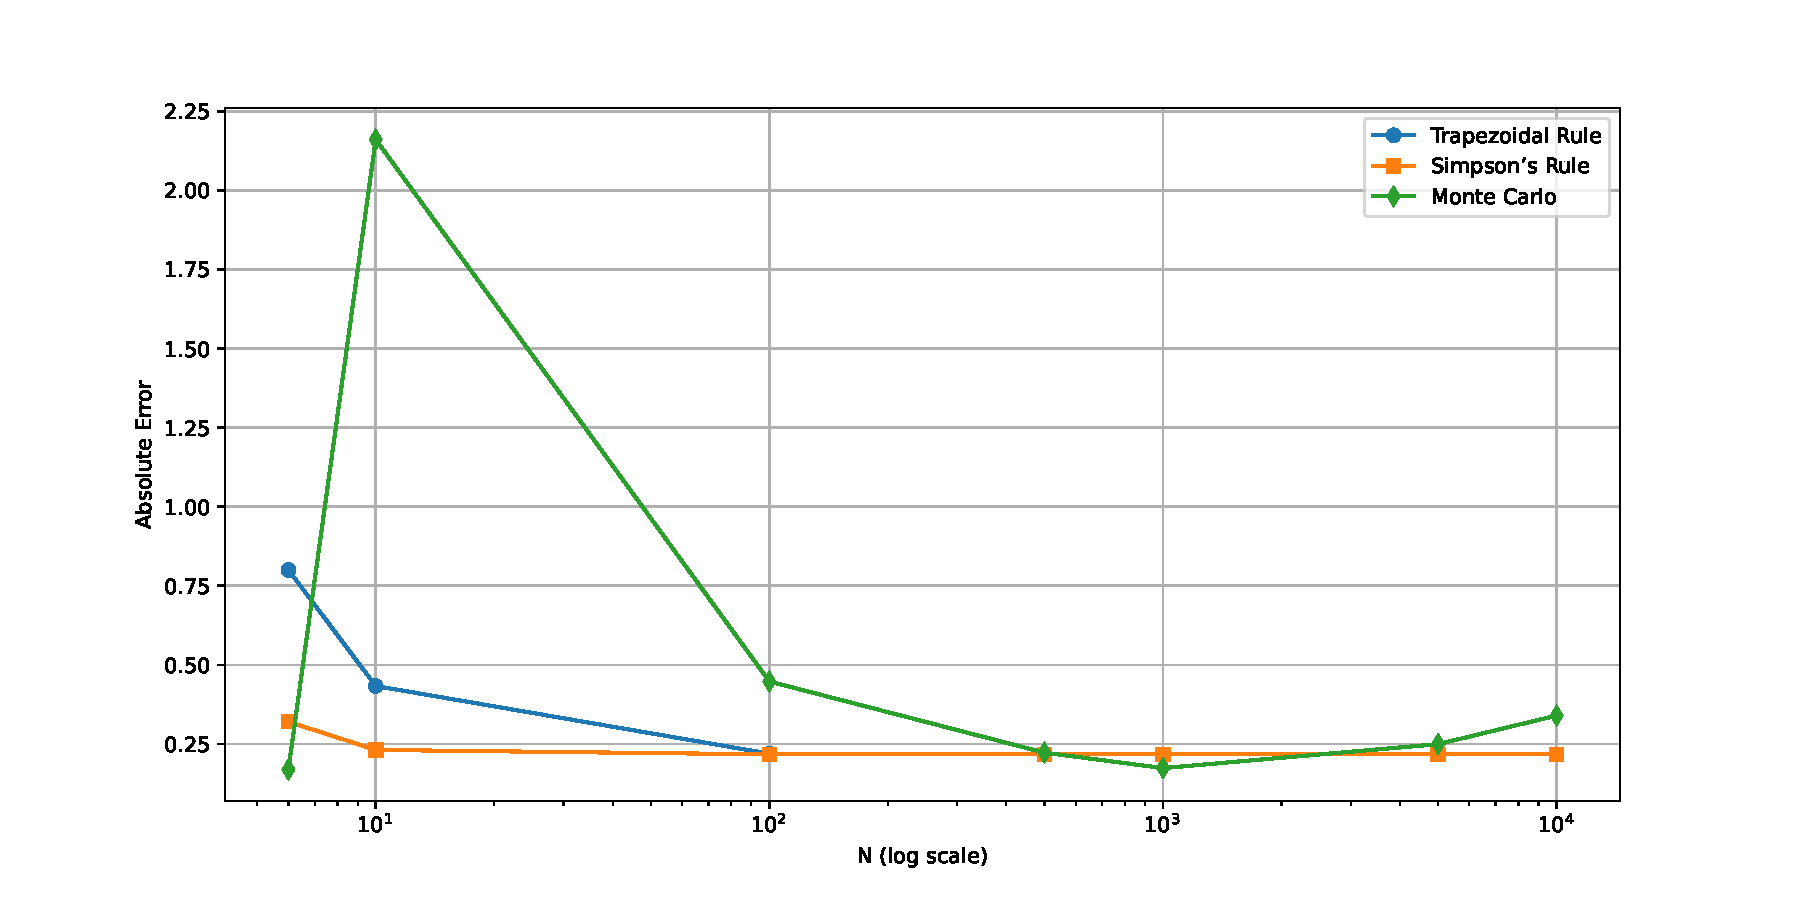
\includegraphics[width=1\linewidth]{../Plots/integrals.pdf}
        \caption{Absolute Errors vs $N$}
        \label{fig:integrals}
    \end{figure}

    \item [4.] Taking $\log$ from both sides of the error terms, we have:
    \begin{align}
        \log E_{\text{Trap}} \sim -\log (n^2)\\
        \log E_{\text{Simp}} \sim -\log (n^4)\\
        \log E_{\text{MC}} \sim -\log (\sqrt{n})
    \end{align}

    It is consistent with the results in the \autoref{fig:integrals}. As we can see, the error of the Simpson's decreasing faster than the other method as $n$ increases.

    \item [5.] Trapezoidal method is simpler ti implement, but it is slower in covergance rather than Simpson method. Simpson method is more precise in lower iterations, bu it requires an even number of intervals. Both of them also require the function to be twice differentiable. For Simpson, it is more restrictive, as it requires the function to be four times differentiable. Monte Carlo method is more flexible, as it does not require the function to be differentiable. However, it is more dependent on the random process, and it is slower than the other methods. It is also more computationally expensive as requires a large number of samples for high accuracy.
\end{enumerate}

\newpage
\section{Portfolio selection and Value at Risk}

In this question, I implictitly assume that returns are normaly distributed and will derive the confidence intervals based on this assumption. Bob can reject that Alice's portfolio were optimaly chosen only if there is no interaction between Alice's MVF and Bob's CI. The results are presented in \autoref{fig:Efficient_Frontier}. I used seed number $\boldsymbol{137}$ for the Monte Carlo simulation.
\begin{figure}[H]
    \centering
    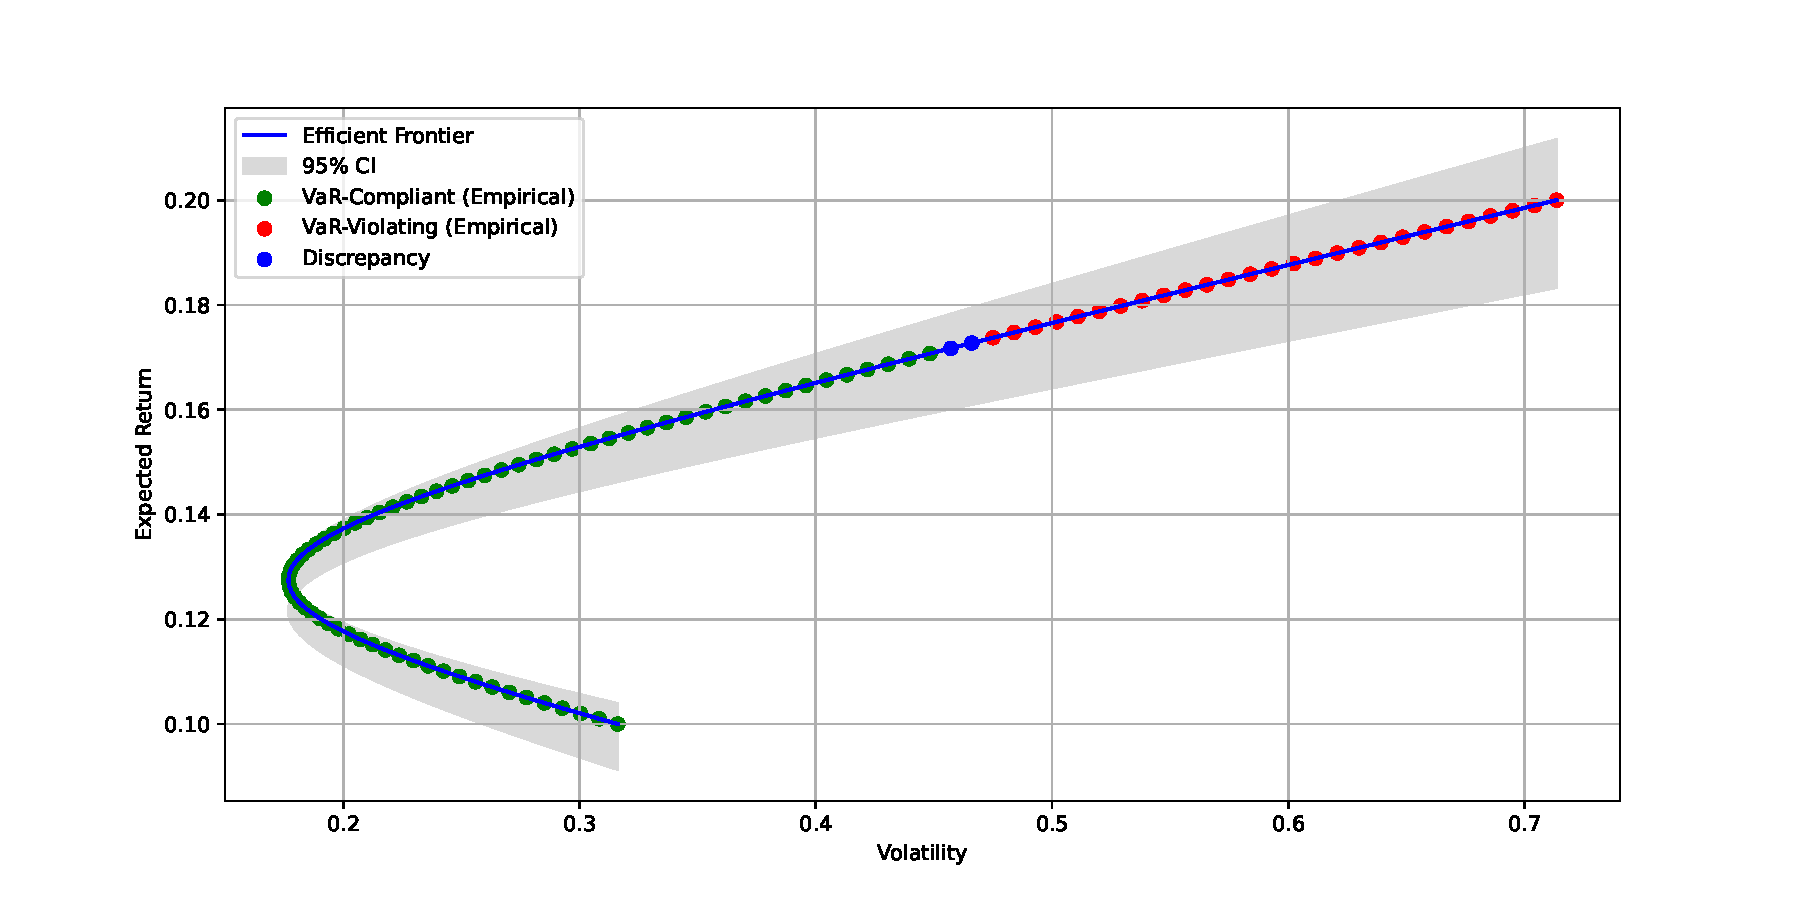
\includegraphics[width=1\linewidth]{../Plots/Efficient_Frontier.pdf}
    \caption{Efficient Frontier with Confidence Intervals and Empirical VaR Compliance}
    \label{fig:Efficient_Frontier}
\end{figure}

To find the upper bound on the volatility we can use the following formula:
\begin{align}
    \sigma_{\text{max}} = \frac{r_{\text{min}}+\bar{V}}{\Phi^{-1}(\lambda)}
\end{align}
where I use the minimum target return as $r_{\text{max}}$. Using this formula we can find the upper bound on the volatility:
\begin{align}
    \sigma_{\text{max}} = 0.3337
\end{align}

Comparing the theoretical and empirical VaR, we need to consider that the theoretical one is not necessarily like the empirical one and that is because the returns are not necessarily normally distributed. The normal distribution is symmetric, but the returns are not necessarily symmetric. In this case, since the distributions of the returns are pretty like each other, the return distribution of Alice is also looks like normal and we have the same VaR-compliant portfolios. The only difference between them is mostly because of the randomness of the Monte Carlo data generation algorithm (blue dots in \autoref{fig:Efficient_Frontier}). However, in general, the theoretical VaR is not necessarily like the empirical VaR. 

The distribution of the returns for Bob's and Alice's are depicted in \autoref{fig:return_distribution}.

\begin{figure}[H]
    \centering
    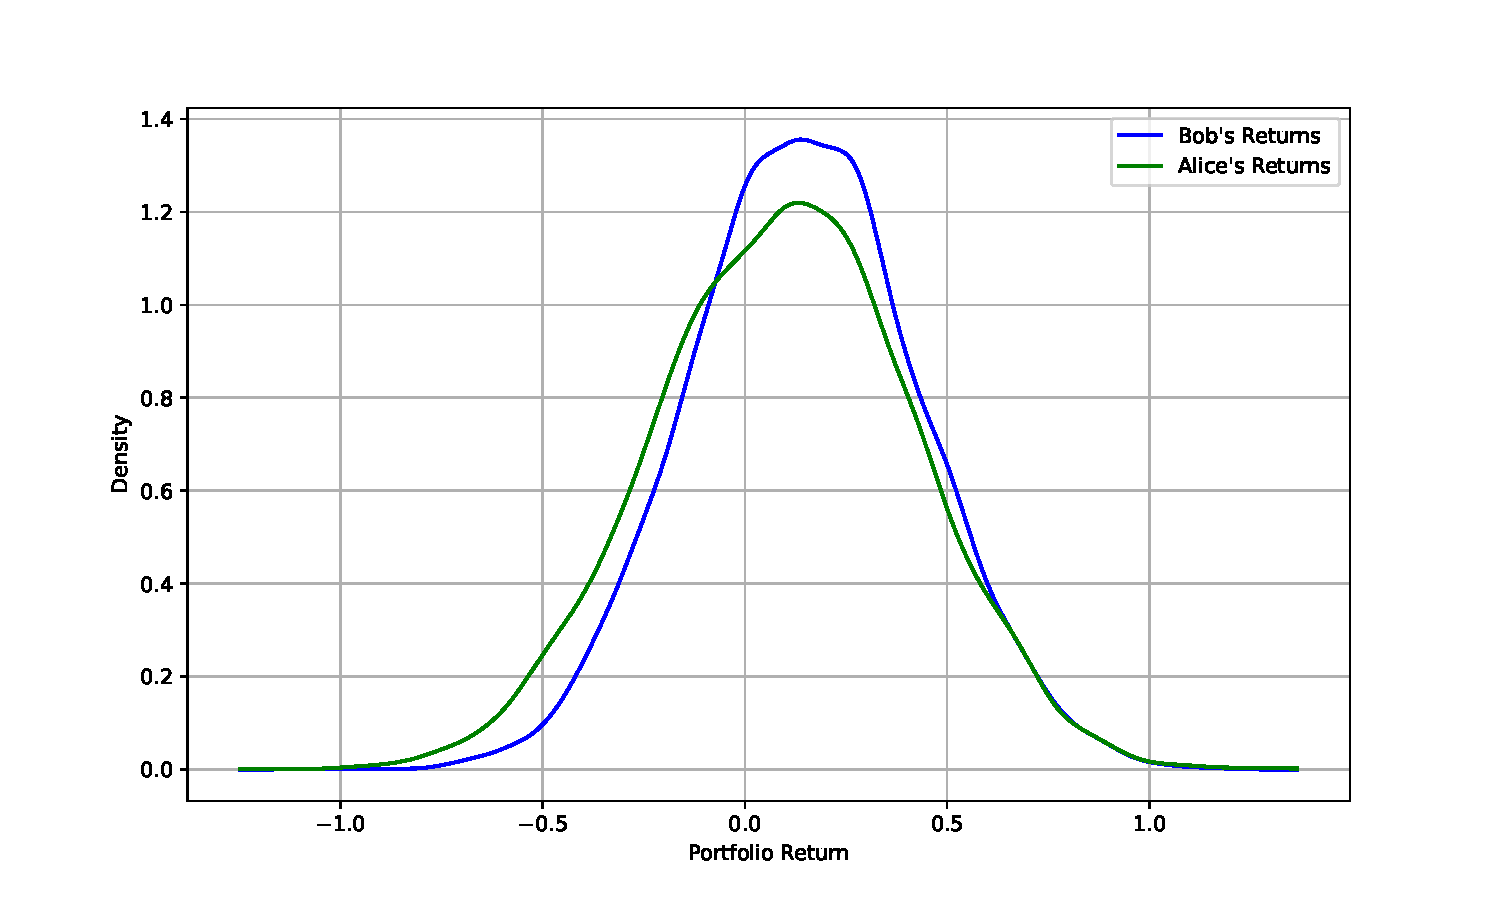
\includegraphics[width=1\linewidth]{../Plots/return_distribution.pdf}
    \caption{Distribution of Bob's and Alice's Returns}
    \label{fig:return_distribution}
\end{figure}






















% \newpage
% \bibliography{ref}


\end{document}